\documentclass[12pt]{article}
\setlength{\oddsidemargin}{0in}
\setlength{\evensidemargin}{0in}
\setlength{\textwidth}{6.5in}
\setlength{\parindent}{0in}
\setlength{\parskip}{\baselineskip}

\usepackage{amsmath,amsfonts,amssymb,bm,graphics,pgfplots,framed,dsfont}
\usepackage[scale=0.75,top=1cm,bottom=3cm]{geometry}

\begin{document}

\textbf{Minh Anh Nguyen }\\
\textbf{Calculus 1 Assignment-}\\
\textbf{Section: 04}\\
\textbf{TA's name: Arthur Huey}

\hrulefill

Section 5.3:

\begin{enumerate}
\setcounter{enumi}{9}
    \item Use the method of cylindrical shells to find the volume generated by rotating the region bounded by the given curves about the y-axis.
    \[y=x^3,y=0,x=1,x=2\]
    \begin{center}
        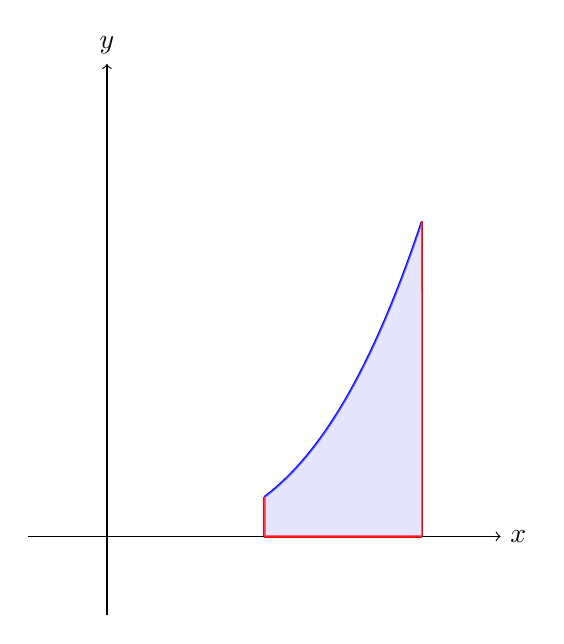
\begin{tikzpicture}[scale=2]
            % Axes
            \draw[->] (-0.5,0) -- (2.5,0) node[right] {$x$};
            \draw[->] (0,-0.5) -- (0,3) node[above] {$y$};
            
            % Curve: y = x^3 (scaled in y-direction)
            \draw[thick,blue] plot[domain=1:2,samples=100] (\x,{0.25*\x^3});
            
            % Lines x=1 and x=2
            \draw[thick,red] (1,0) -- (1,0.25) ;
            \draw[thick,red] (2,0) -- (2,2) ;
            
            % Line y=0
            \draw[thick,red] (1,0) -- (2,0);
            
            % Shaded region
            \fill[blue!20,opacity=0.5] 
                (1,0) -- plot[domain=1:2,samples=100] (\x,{0.25*\x^3}) -- (2,0) -- cycle;
        \end{tikzpicture}
    \end{center}
\end{enumerate}
\end{document}